\section{Usage Scenario In Practice}

Currently \Klang{} is being used to analyze models created for the
NASA Europa Clipper Mission. In Section~\ref{sec:introduction}, we
briefly introduced this usage scenario (shown in
Figure~\ref{fig:k}). The typical scenario involves modelers creating
SysML diagrams in MagicDraw and saving them to a central model
repository. This database of models is accessible through a REST
API. The input to the REST API is a unique identifier for a node in
the model, and the result is a list of all the nodes that belong under
that node (as an array of JSON objects). Typically, the identifier of
a {\em package} node in the model is used as input to the REST API,
which in return gives us all the classes, constraints, and properties
that have been defined in the package. The \Klang{} tool chain takes
this input and converts each node in the list of nodes to a
corresponding \Klang{} AST object. Since the list of nodes received
from the REST API is completely unordered and unstructured, we perform
multiple passes on the list of nodes. The first pass is performed to
create the list of classes in the model, followed by passes to
populate properties and constraints in each class. Once the \Klang{}
model has been constructed, the \Klang{} tool chain proceeds normally
with type checking and SMT analysis. Currently this scenario is based
on a {\em pull} methodology where a modeler has to initiate the
\Klang{} based translation and analysis. In the future, we plan on
automating this effort and have it be executed on a regular cadence
with results made available through the model database to a web
application.

\begin{figure*}
\centering
\fbox{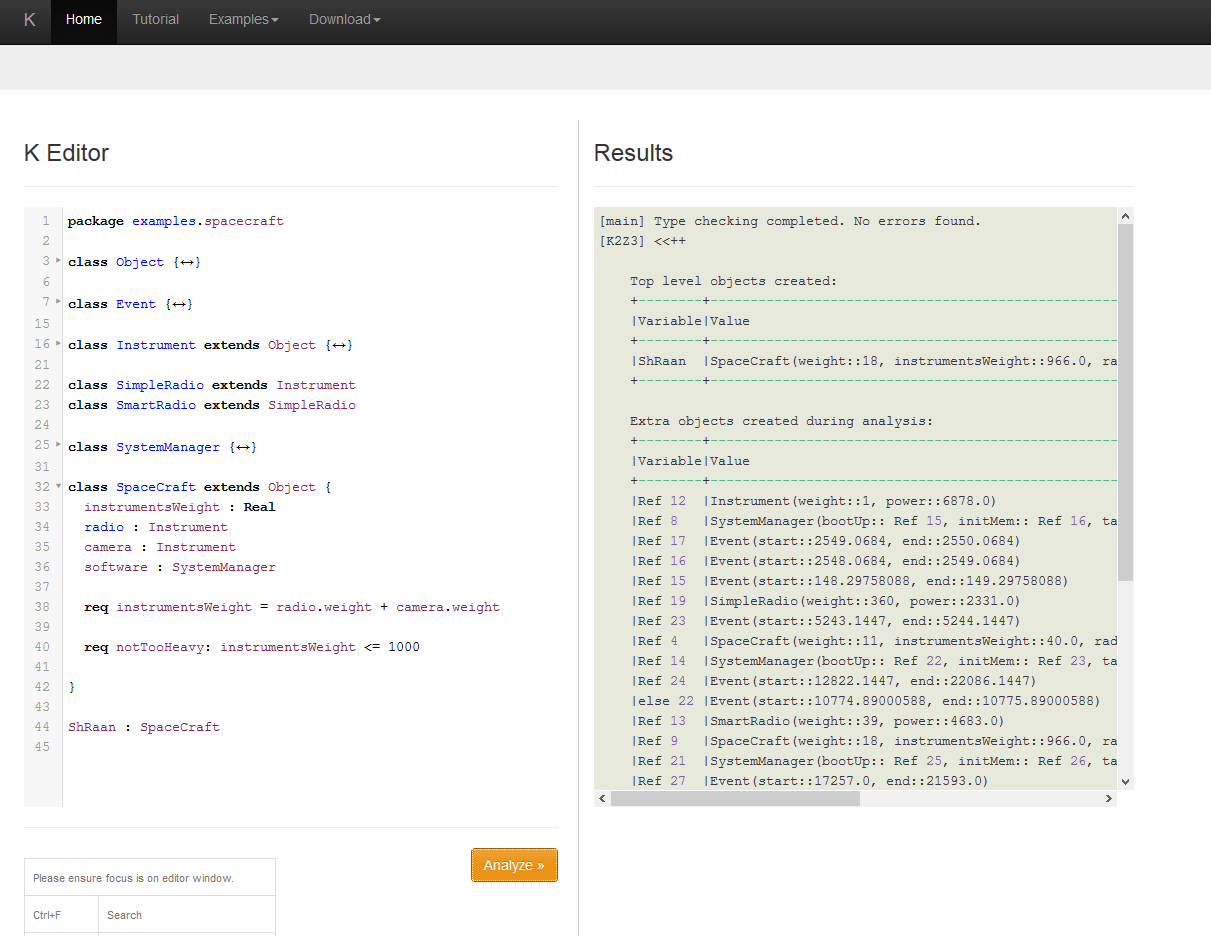
\includegraphics[scale=0.3]{kweb.png}}
\caption{\Klang{} editor in the browser.}
\label{fig:k}
\end{figure*}

A second common scenario for using \Klang{} is via the web browser. We
have created a simple HTML based \Klang{} code editor along with the
functionality to invoke the type checker and SMT analysis via the web
browser. This page is used for purposes of teaching, learning,
exploring, and prototyping with \Klang{}. The web page also provides a
tutorial, documentation, and \Klang{} examples as a guide. 

